\hl{L3:NetworkEmbedding} 
\hlgreen{NE: Node}Project nodes in a unified vector space to preserve the network similarity. Workflow of Learning NE: \hlpurple{encoder} projects nodes to embeddings; Define the \hlpurple{similarity} function for network structures Euclidean/Cosine distance; \hlpurple{decoder} recover; Optimize parameters to minimize the reconstruction loss.
$L = \sum_{u,v \in \mathcal{D}} \ell( \mathrm{DEC}(z_u, z_v),\mathrm{Similarity}(u,v))$
\hlorange{homogeneous or heterogeneous} In a homogeneous graph, all the nodes represent instances of the same type and all the edges represent relations of the same type. in a heterogeneous graph, the nodes and edges can be of different types.
\hlgreen{NE: node relationship} \hlpurple{co-occurrence}: random walk; \hlpurple{proximity}(nearness in space, time, or relationship.): 1st,2nd order.
\hlpurple{word2vec} maximize the probability of co-occurrence of close words for each word.
\hlorange{random walk: Advantages} 
\hlpurple{Expressivity:} Flexible stochastic definition of node similarity that incorporates both local and higher-order neighborhood information. If a random walk starting from node \( u \) visits \( v \) with high probability, \( u \) and \( v \) are considered similar (this reflects high-order multi-hop information).
\hlpurple{Efficiency:} Do not need to consider all node pairs when training; consider pairs that co-occur on random walks.
\hlblue{EG: v1-v2-v3-v4-v5-v6} 
\begin{tabular}{|c|c|}
\hline
\textbf{node} & \textbf{context nodes} \\
\hline
$v1$ & $v2,v3$ \\
$v2$ & $v1,v3,v4$ \\
$v3$ & $v1,v2,v4,v5$ \\
$v4$ & $v2,v3,v5,v6$ \\
\hline
\end{tabular} 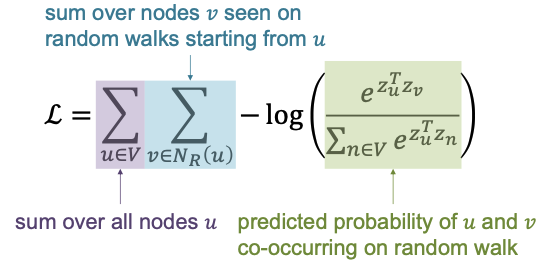
\includegraphics[height=0.045\textwidth]{figs/l3-1.png}
\hlorange{deepwalk} predict the context nodes with embedings, Maximize conditional probability:\(p(v_{context} | v_{cen})\)
\hlorange{Limitation:} Nested sum over all nodes results in \( O(|V^{2}|) \) complexity.
\hlorange{Negative Sampling}
\(L=-\log\left(\frac{\exp(\mathbf{z_u^T z_v})}{\sum_{n \in V} \exp(\mathbf{z_u^T z_n})}\right) \approx \log\left(\sigma(\mathbf{z_u^T z_v})\right) + \sum_{i=1}^{k} \log\left(\sigma(-\mathbf{z_u^T z_{n_i}})\right)\) 
% \textcolor{red}{spend more time} 
another way to improve efficiency is 
\hlorange{Hierarchical Softmax}: optimize embeddings with Hierarchical Softmax using Stochastic Gradient Descent.
\hlorange{Node2Vec} difference between deepwalk: Develop biased second order random walk  \(\mathcal{R}\) to generate network neighborhood  \(\mathcal{N}_0(u) \text{ of node } u.\)
\hlorange{Biased walks:}
To trade off between local and global views of the network.
1. Local view: visited through BFS. (purple)
2. Global view: visited through DFS. (orange)
\hlorange{N-order Proximity} First order proximity: for two nodes connected by edge. Second order proximity: for 2-hop neighbor. Optimize two decoder separately using KL-divergence. node 6, 7: 1st order; node 6, 5 2nd order. dtx is the distance from t to x.
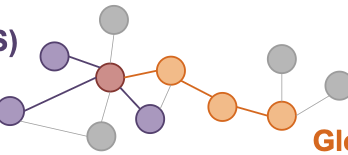
\includegraphics[height=0.03\textwidth]{figs/l3-4.png}
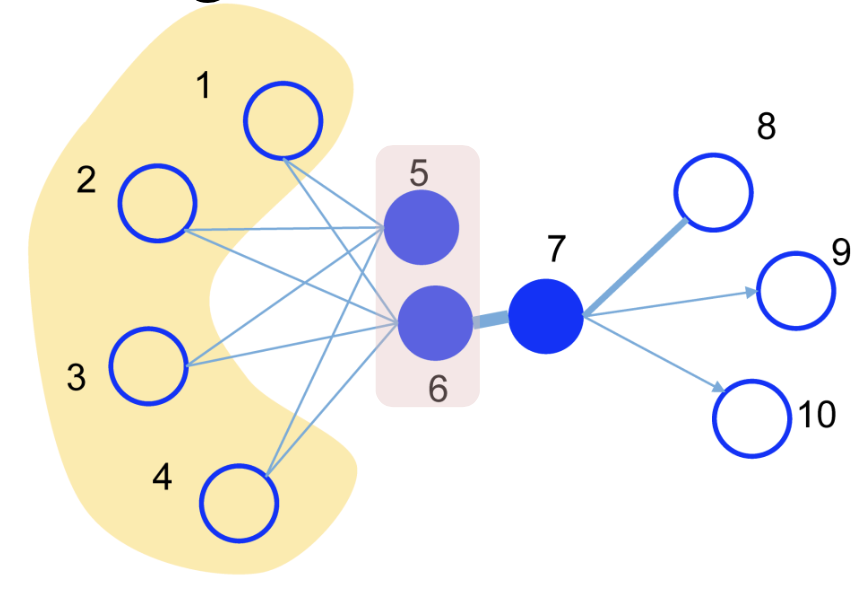
\includegraphics[height=0.03\textwidth]{figs/l3-2.png}
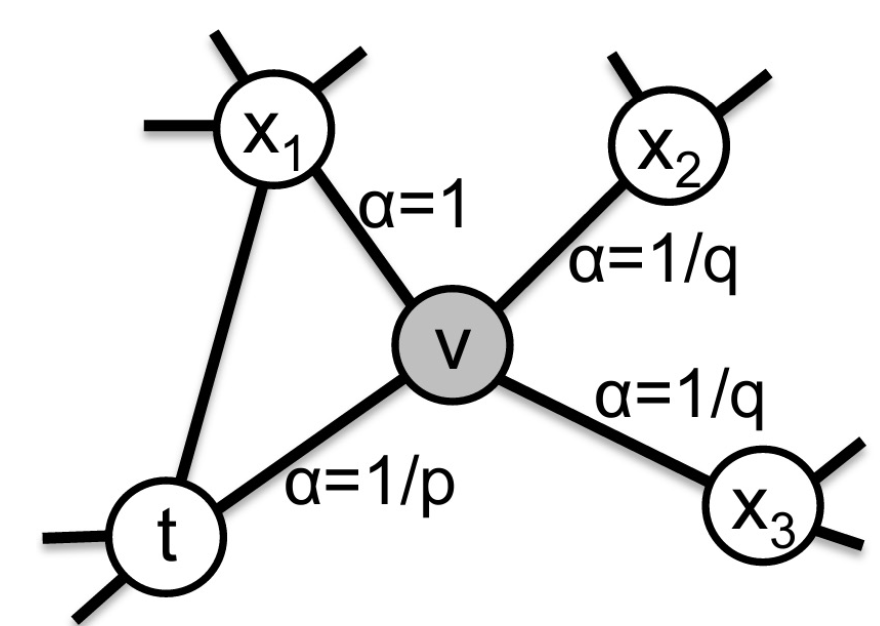
\includegraphics[height=0.03\textwidth]{figs/l3-3.png}
\(a_{pq}(t, x) = 
\begin{cases} 
\frac{1}{p} & \text{if } d_{tx} = 0 \\
1 & \text{if } d_{tx} = 1 \\
\frac{1}{a} & \text{if } d_{tx} = 2 \\
\end{cases}
\)
Smaller p result in sampled neighbors around t (BFS), smaller q result in sampled neighbors away from t (DFS)
\hlgreen{NetworkEmbedding: structural relationship} preserving structural feature: Microscopic and Mesoscopic.
\hlorange{struc2vec}preserve microscopic node similarity. Suppose u v are two distant nodes; They are structural similar, but hard to measure. 1. Measure structural role similarity g(vi, vj); 2. build a new graph; 3. deep walk -> node embedding.
\hlorange{Modularized Nonnegative Matrix Factorization (M-NMF)} preserve mesoscopic community structure.
Exploit the consensus relationship between the representations of nodes and community structure.
Joint optimization: a. NMF based representation learning model; b. Modularity based community detection model.
\hlorange{summary}Network embedding on simple networks: preserving node/structure based similarity. Preserving \hlpurple{node} relationship: DeepWalk, Node2Vec; Preserving \hlpurple{structure} information: Microscopic (close neighbors): Struc2Vec; Mesoscopic (community): M-NMF

\hl{L4:GNN1} \hlpurple{RELU}\(f(x) = \max(0, x)\) \hlpurple{Sigmoid}\(f(x) = \frac{1}{{1 + e^{-x}}}\)
\hlorange{Feedforward Neural Networks for graph}Problem: 1. Problems:O(|V|) parameters, 2.Not applicable to graphs of different sizes 2. Sensitive to node ordering
\hlorange{CNN for graph}Problem: 1. Problems: 1. There is no notion of sliding window on graph. 2. CNNs are sensitive to input size and order, whereas graphs are variable in size and permutation invariant. 
\hlorange{Permutation Invariance and Permutation Equivariance} FNNs, CNNs, are Not permutation invariant / equivariant! Graph Neural Networks should be permutation invariant and equivariant. Given arbitrary order plan, equivariant same as the order plan, invariant as the whole graph. Then, if \( f(Ai,Fi) = f(Aj,Fj) \) for any order plan \( i \) and \( j \), we formally say \( f \) is a \hlpurple{permutation invariant} function. If the output vector of a node at the same position in the graph remains unchanged for any order plan, we say f is \hlpurple{permutation equivariant}
\hlorange{Framework for Node level tasks} a composition of graph convolution and non-linear activation layers
\hlorange{Framework for Graph level tasks} graph convolution and pooling layer (Summarize node features to generate the representation for the subgraphs or the entire graph).


